\documentclass[11pt]{article}

\usepackage[utf8]{inputenc}
\usepackage[T1]{fontenc}
\usepackage[spanish,es-nodecimaldot]{babel}
\usepackage{mathptmx}
\usepackage[margin=2.3cm]{geometry}
\usepackage{microtype}
\usepackage{amsmath}
\usepackage{graphicx}
\graphicspath{{figuras/}}
\usepackage{enumitem}
\usepackage{titlesec}
\usepackage{parskip}
\usepackage{float}

\titleformat{\section}{\normalfont\bfseries\large}{}{0pt}{}
\titlespacing*{\section}{0pt}{12pt}{4pt}
\titleformat{\subsection}{\normalfont\bfseries}{}{0pt}{}
\titlespacing*{\subsection}{0pt}{8pt}{2pt}
\setlist[itemize]{leftmargin=1.2em,itemsep=2pt,topsep=2pt}
\setlist[enumerate]{leftmargin=1.6em,itemsep=3pt,topsep=3pt}
\pagestyle{empty}
\setlength{\parskip}{5pt}
\hyphenpenalty=10000
\exhyphenpenalty=10000
\emergencystretch=2em

\begin{document}

\begin{center}
	{\small SMAII, Redes Complejas Multicapa}\\[6pt]
	{\Large\bfseries Proyecto final: sección de Resultados}\\[3pt]
	{\normalsize Efecto de una campaña sobre la opinión colectiva y predicción de su conveniencia}\\[4pt]
	{\small Noviembre de 2026}
\end{center}

\section*{Integrantes del equipo}
\begin{itemize}
	\item Jorge Miyoshi Mikami Alonso
	\item Luis Manuel Reyes Colín
\end{itemize}

\section*{Resultados}

Aquí mostramos lo que obtuvimos en las simulaciones, en el orden de los objetivos particulares. La
discusión va en la siguiente sección. Si no se dice otra cosa, cada simulación tiene $N=1000$ personas,
8 contactos por persona en la capa 1, 4 en la capa 2, y al inicio el $10\%$ de las personas está activo.
Llamamos \emph{fracción junto a la campaña} ($S_m$) a la fracción de personas que al final quedó a menos
de $0.05$ de $x_m$, y \emph{grupo de opinión} a un conjunto de personas con opiniones casi iguales que
reúne al menos al $1\%$ de la población.

\subsection*{1. Validación del modelo de opinión}

Primero corrimos el modelo sin red y sin conducta, con 100 personas que pueden hablar con todos. La
Figura~\ref{fig:val_hist} muestra un ejemplo y la Figura~\ref{fig:val} los cuatro escenarios de
Pansanella \emph{et al.}

\begin{figure}[H]
	\centering
	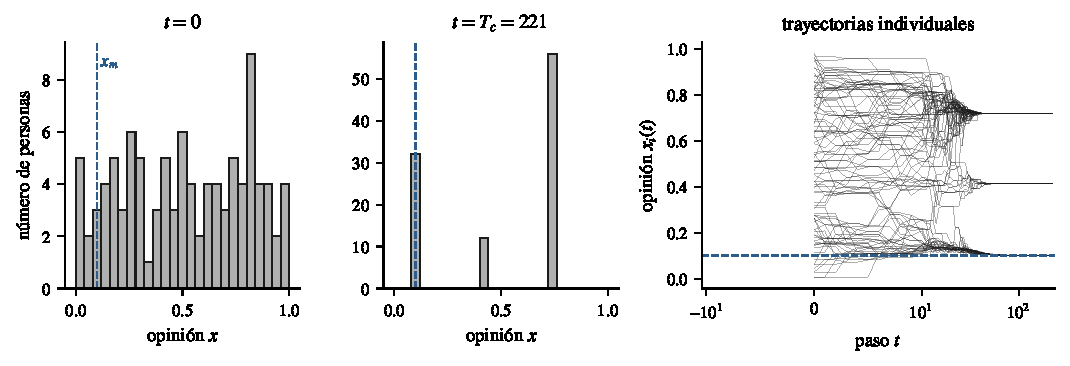
\includegraphics[width=\textwidth]{validacion_histogramas}
	\caption{Ejemplo de validación. Izquierda y centro: opiniones al inicio y al final. Derecha: opinión de
	cada persona a lo largo del tiempo. La línea discontinua es la campaña. Parámetros: $N=100$, todos
	con todos, sin capa de conducta, $\epsilon=0.2$, $\gamma=1$, $p_m=0.1$, $x_m=0.1$.}
	\label{fig:val_hist}
\end{figure}

\begin{figure}[H]
	\centering
	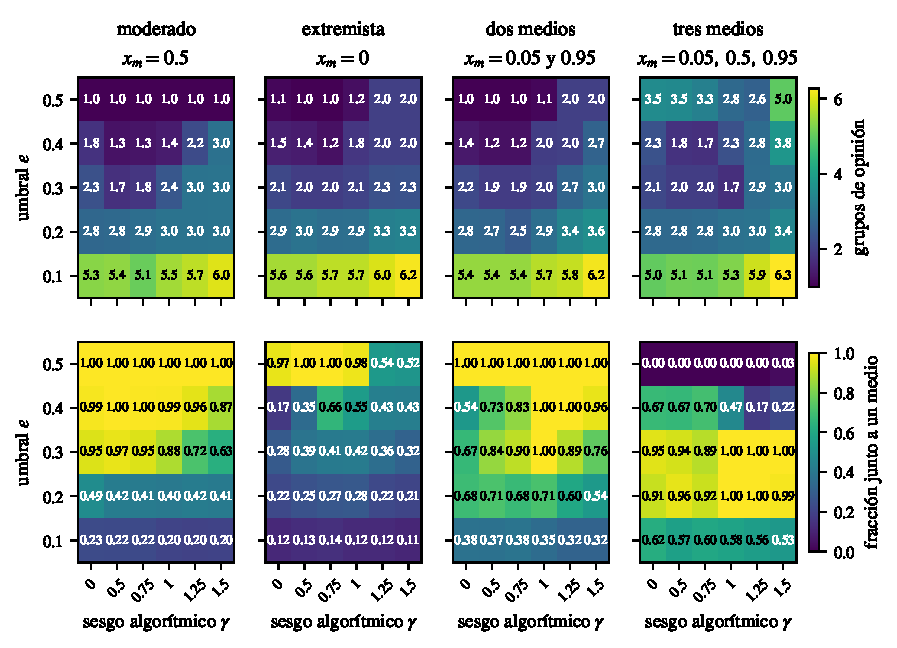
\includegraphics[width=\textwidth]{s_validacion}
	\caption{Validación en los cuatro escenarios de medios. Arriba: número de grupos de opinión al final.
	Abajo: fracción de personas que terminó a menos de $0.05$ de algún medio. Cada celda es el promedio de
	30 corridas. Parámetros: $N=100$, todos con todos, sin capa de conducta, $p_m=0.1$, opiniones
	iniciales al azar entre 0 y 1.}
	\label{fig:val}
\end{figure}

\subsection*{2. Red de dos capas}

El Cuadro~\ref{tab:red} tiene las medidas básicas de las redes y la Figura~\ref{fig:grado} sus
distribuciones de grado. La Figura~\ref{fig:red} dibuja las dos capas al inicio y al final de una
simulación pequeña. En promedio, las dos capas comparten 16 aristas (menos del $1\%$).

\begin{table}[H]
	\centering
	\small
	\begin{tabular}{lcccc}
		\hline
		Capa & Aristas & Grado promedio & Agrupamiento & Camino promedio \\
		\hline
		1, Erd\H{o}s--Rényi & 4007 & 8.0 & 0.008 & 3.55 \\
		1, Barabási--Albert & 3984 & 8.0 & 0.025 & 3.18 \\
		2, aleatoria con grado 4 & 2000 & 4.0 & 0.004 & 5.64 \\
		\hline
	\end{tabular}
	\caption{Medidas de las capas con $N=1000$ (promedio de 10 redes de cada tipo).}
	\label{tab:red}
\end{table}

\begin{figure}[H]
	\centering
	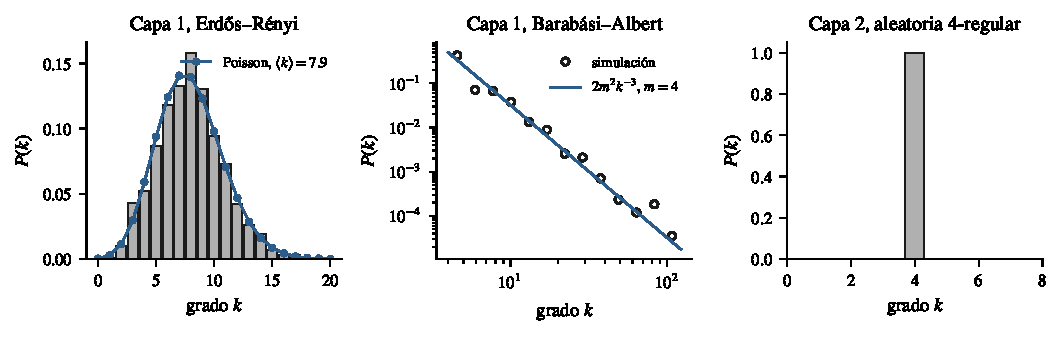
\includegraphics[width=\textwidth]{distribucion_grado}
	\caption{Distribución de grado (cuántas personas tienen $k$ contactos) para una red de cada tipo con
	$N=1000$. En Erd\H{o}s--Rényi se compara con una Poisson y en Barabási--Albert con una ley de
	potencia $k^{-3}$ (ejes logarítmicos).}
	\label{fig:grado}
\end{figure}

\begin{figure}[H]
	\centering
	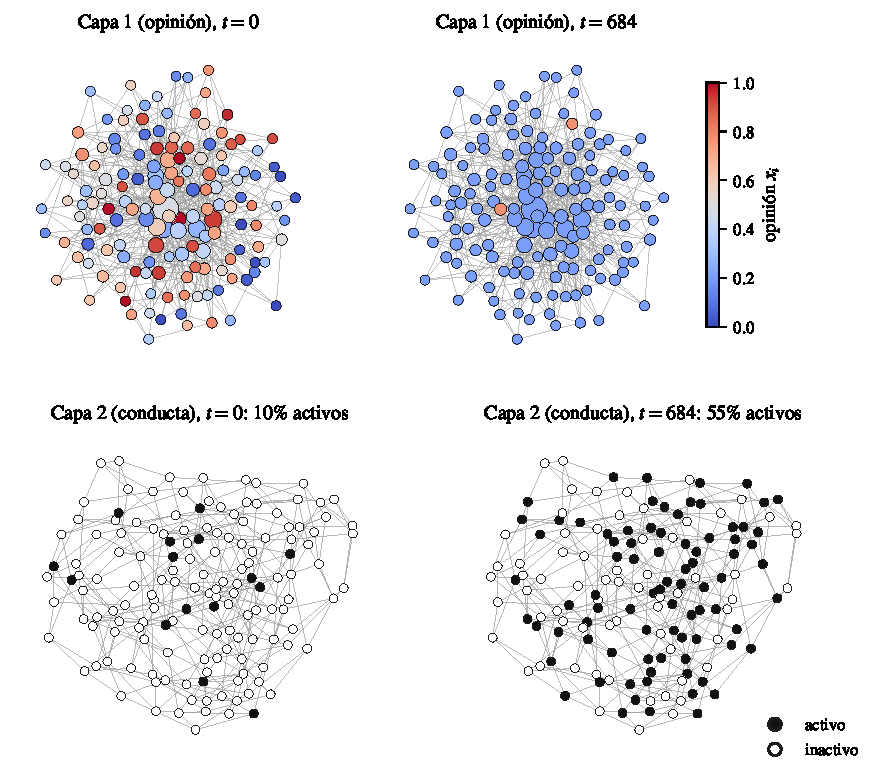
\includegraphics[width=0.88\textwidth]{red_inicio_final}
	\caption{Las dos capas al inicio (izquierda) y al final (derecha) de una simulación pequeña. Arriba, el
	color es la opinión y el tamaño el número de contactos; abajo, negro es activo y blanco inactivo.
	Parámetros: $N=150$, capa 1 Barabási--Albert, $\epsilon=0.3$, $\gamma=0.75$, $p_m=0.2$, $x_m=0.2$,
	$\alpha=1$.}
	\label{fig:red}
\end{figure}

\subsection*{3. Evolución en el tiempo}

La Figura~\ref{fig:tiempo} sigue un mismo escenario con y sin campaña. Con campaña, la opinión
promedio terminó en $0.21$ y la fracción activa en $0.49$; sin campaña, en $0.50$ y $0.19$.

\begin{figure}[H]
	\centering
	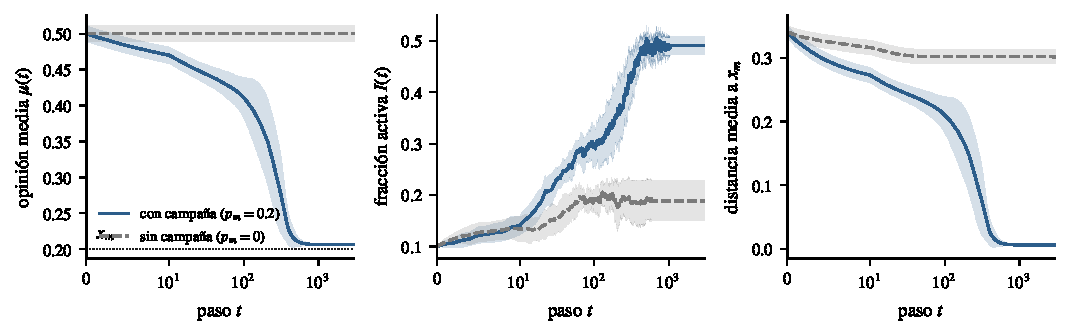
\includegraphics[width=\textwidth]{evolucion_temporal}
	\caption{Opinión promedio, fracción de activos y distancia promedio a la campaña en el tiempo. La línea
	es el promedio de 10 corridas y la franja su desviación estándar. Parámetros: capa 1 Barabási--Albert,
	$\epsilon=0.3$, $\gamma=0.75$, $\alpha=1$, $x_m=0.2$; con campaña $p_m=0.2$ (continua) y sin campaña
	(discontinua).}
	\label{fig:tiempo}
\end{figure}

\subsection*{4. Barrido de parámetros}

La Figura~\ref{fig:mapas} es un mapa de calor como los de Pansanella \emph{et al.}, ahora con red y con
la capa de conducta. El Cuadro~\ref{tab:esc} muestra cuatro escenarios concretos y la
Figura~\ref{fig:alpha} qué pasa con la fracción de activos al cambiar $\alpha$.

\begin{figure}[H]
	\centering
	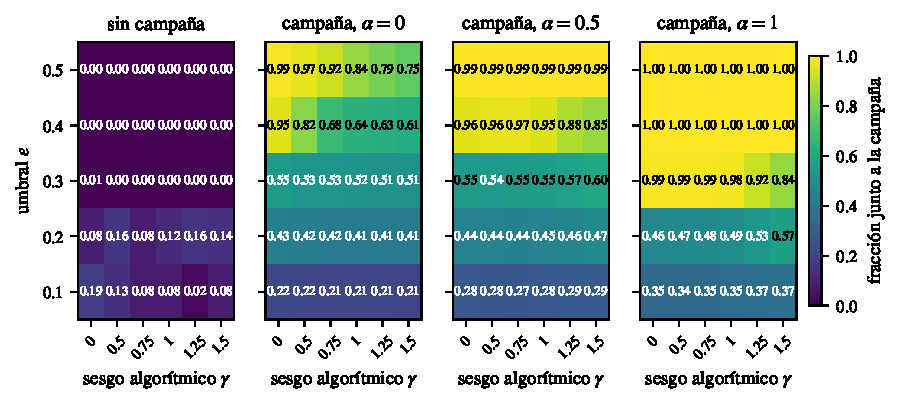
\includegraphics[width=\textwidth]{s_mapas}
	\caption{Fracción junto a la campaña según la apertura $\epsilon$ y el sesgo $\gamma$, sin campaña y con
	campaña para tres valores de $\alpha$. Cada celda es el promedio de 10 corridas. Parámetros: capa 1
	Barabási--Albert, $x_m=0.2$, $p_m=0.3$ (o $0$ sin campaña).}
	\label{fig:mapas}
\end{figure}

\begin{table}[H]
	\centering
	\small
	\begin{tabular}{ccccl}
		\hline
		$(\epsilon,\gamma,\alpha,p_m)$ & Grupos & $S_m$ & Activos al final & Estado \\
		\hline
		$(0.2,\,0,\,0,\,0.1)$ & 2.9 & 0.45 & 0.24 & polarización \\
		$(0.2,\,1,\,0.5,\,0.1)$ & 2.6 & 0.45 & 0.23 & polarización \\
		$(0.4,\,0.5,\,1,\,0.3)$ & 1.0 & 1.00 & 0.49 & consenso \\
		$(0.4,\,1.5,\,1,\,0.5)$ & 1.0 & 1.00 & 0.50 & consenso \\
		\hline
	\end{tabular}
	\caption{Estado final en cuatro escenarios (promedio de 10 corridas). Parámetros: capa 1
	Barabási--Albert, $x_m=0.2$.}
	\label{tab:esc}
\end{table}

\begin{figure}[H]
	\centering
	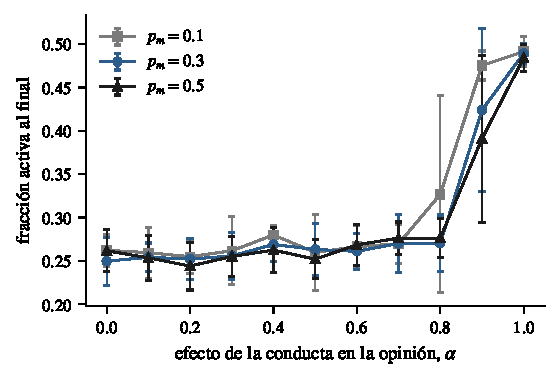
\includegraphics[width=0.55\textwidth]{s_alpha}
	\caption{Fracción de activos al final contra $\alpha$ para tres exposiciones a la campaña. Promedio y
	desviación estándar de 10 corridas. Parámetros: capa 1 Barabási--Albert, $\epsilon=0.3$,
	$\gamma=0.75$, $x_m=0.2$.}
	\label{fig:alpha}
\end{figure}

Para todo el barrido clasificamos el final de cada corrida como \emph{consenso} (un grupo con al menos el
$90\%$ de las personas), \emph{polarización} (dos grupos grandes y separados) o \emph{fragmentación}
(cualquier otro caso). La Figura~\ref{fig:estados} muestra cuántas corridas cayeron en cada caso. En
total corrimos 12\,960 combinaciones, y el $99.9\%$ se estabilizó antes del límite de $10^4$ pasos.

\begin{figure}[H]
	\centering
	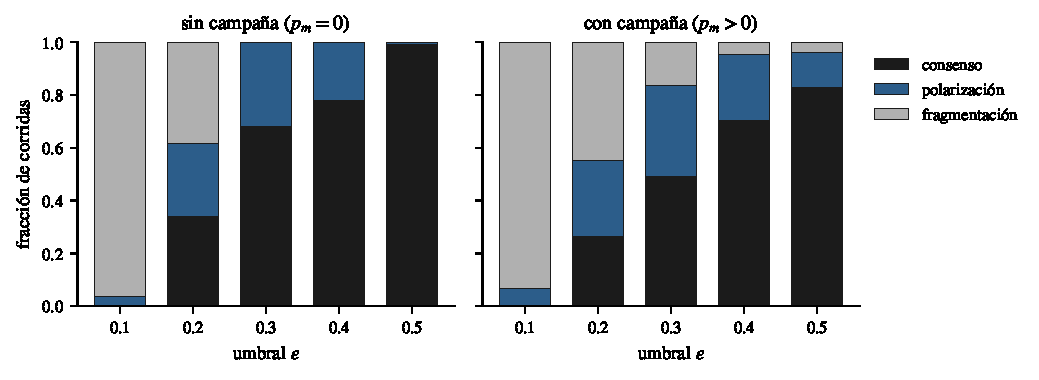
\includegraphics[width=0.85\textwidth]{estados_finales}
	\caption{Fracción de corridas que terminó en consenso, polarización o fragmentación, según $\epsilon$,
	sin campaña (izquierda) y con campaña (derecha). Junta las dos redes, las cuatro poblaciones
	iniciales y todos los valores de $\gamma$, $p_m$, $\alpha$ y $x_m\in\{0,\,0.2,\,0.5\}$ (una corrida
	por combinación).}
	\label{fig:estados}
\end{figure}

\subsection*{5. Clasificación de las campañas y predictor}

Comparamos cada corrida con campaña contra la misma población sin campaña y le pusimos una etiqueta con
las reglas de la Metodología. De las 10\,800 corridas con campaña, 6\,597 salieron favorables, 3\,010
neutras y 1\,193 contraproducentes. La Figura~\ref{fig:etiquetas} muestra cómo se reparten según la
campaña.

\begin{figure}[H]
	\centering
	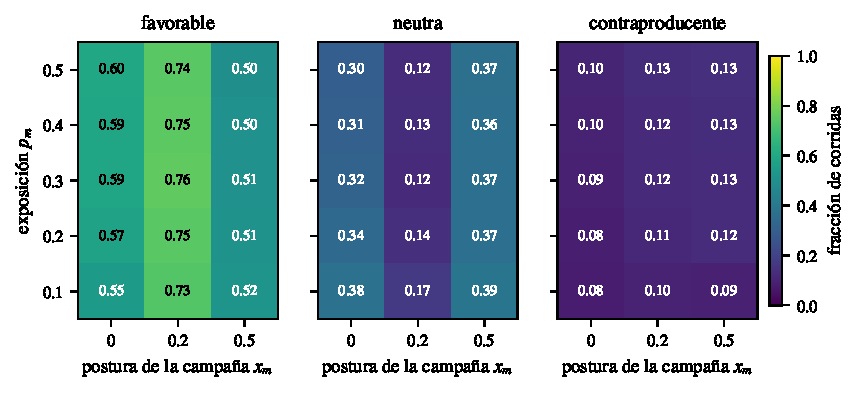
\includegraphics[width=\textwidth]{s_etiquetas}
	\caption{Fracción de corridas con cada etiqueta según la postura $x_m$ y la exposición $p_m$ de la
	campaña. Cada celda junta las dos redes, las cuatro poblaciones iniciales y todos los valores de
	$\epsilon$, $\gamma$ y $\alpha$.}
	\label{fig:etiquetas}
\end{figure}

Para el predictor apartamos el $20\%$ de las combinaciones de parámetros (2\,160 corridas) y entrenamos
con el resto. El Cuadro~\ref{tab:ml} compara los modelos, la Figura~\ref{fig:conf} muestra los aciertos
del mejor y la Figura~\ref{fig:arbol} el árbol de decisión pequeño.

\begin{table}[H]
	\centering
	\small
	\begin{tabular}{lcc}
		\hline
		Modelo & Exactitud & F1 \\
		\hline
		Siempre decir ``favorable'' (referencia) & 0.64 & 0.26 \\
		Regresión logística & 0.63 & 0.41 \\
		Árbol de decisión (4 preguntas) & 0.83 & 0.73 \\
		Bosque aleatorio & 0.95 & 0.91 \\
		\emph{Gradient boosting} & \textbf{0.96} & \textbf{0.93} \\
		\hline
	\end{tabular}
	\caption{Desempeño de los modelos en las 2\,160 corridas de prueba, que no se usaron para entrenar.
	El F1 es el promedio de las tres etiquetas.}
	\label{tab:ml}
\end{table}

\begin{figure}[H]
	\centering
	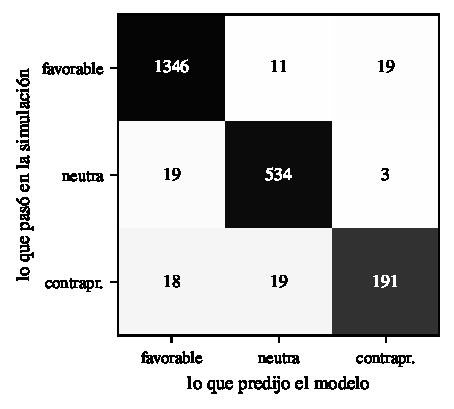
\includegraphics[width=0.45\textwidth]{s_confusion}
	\caption{Matriz de confusión del \emph{gradient boosting} en las 2\,160 corridas de prueba. Cada número
	es cuántas corridas tenían la etiqueta del renglón y el modelo les asignó la de la columna.}
	\label{fig:conf}
\end{figure}

\begin{figure}[H]
	\centering
	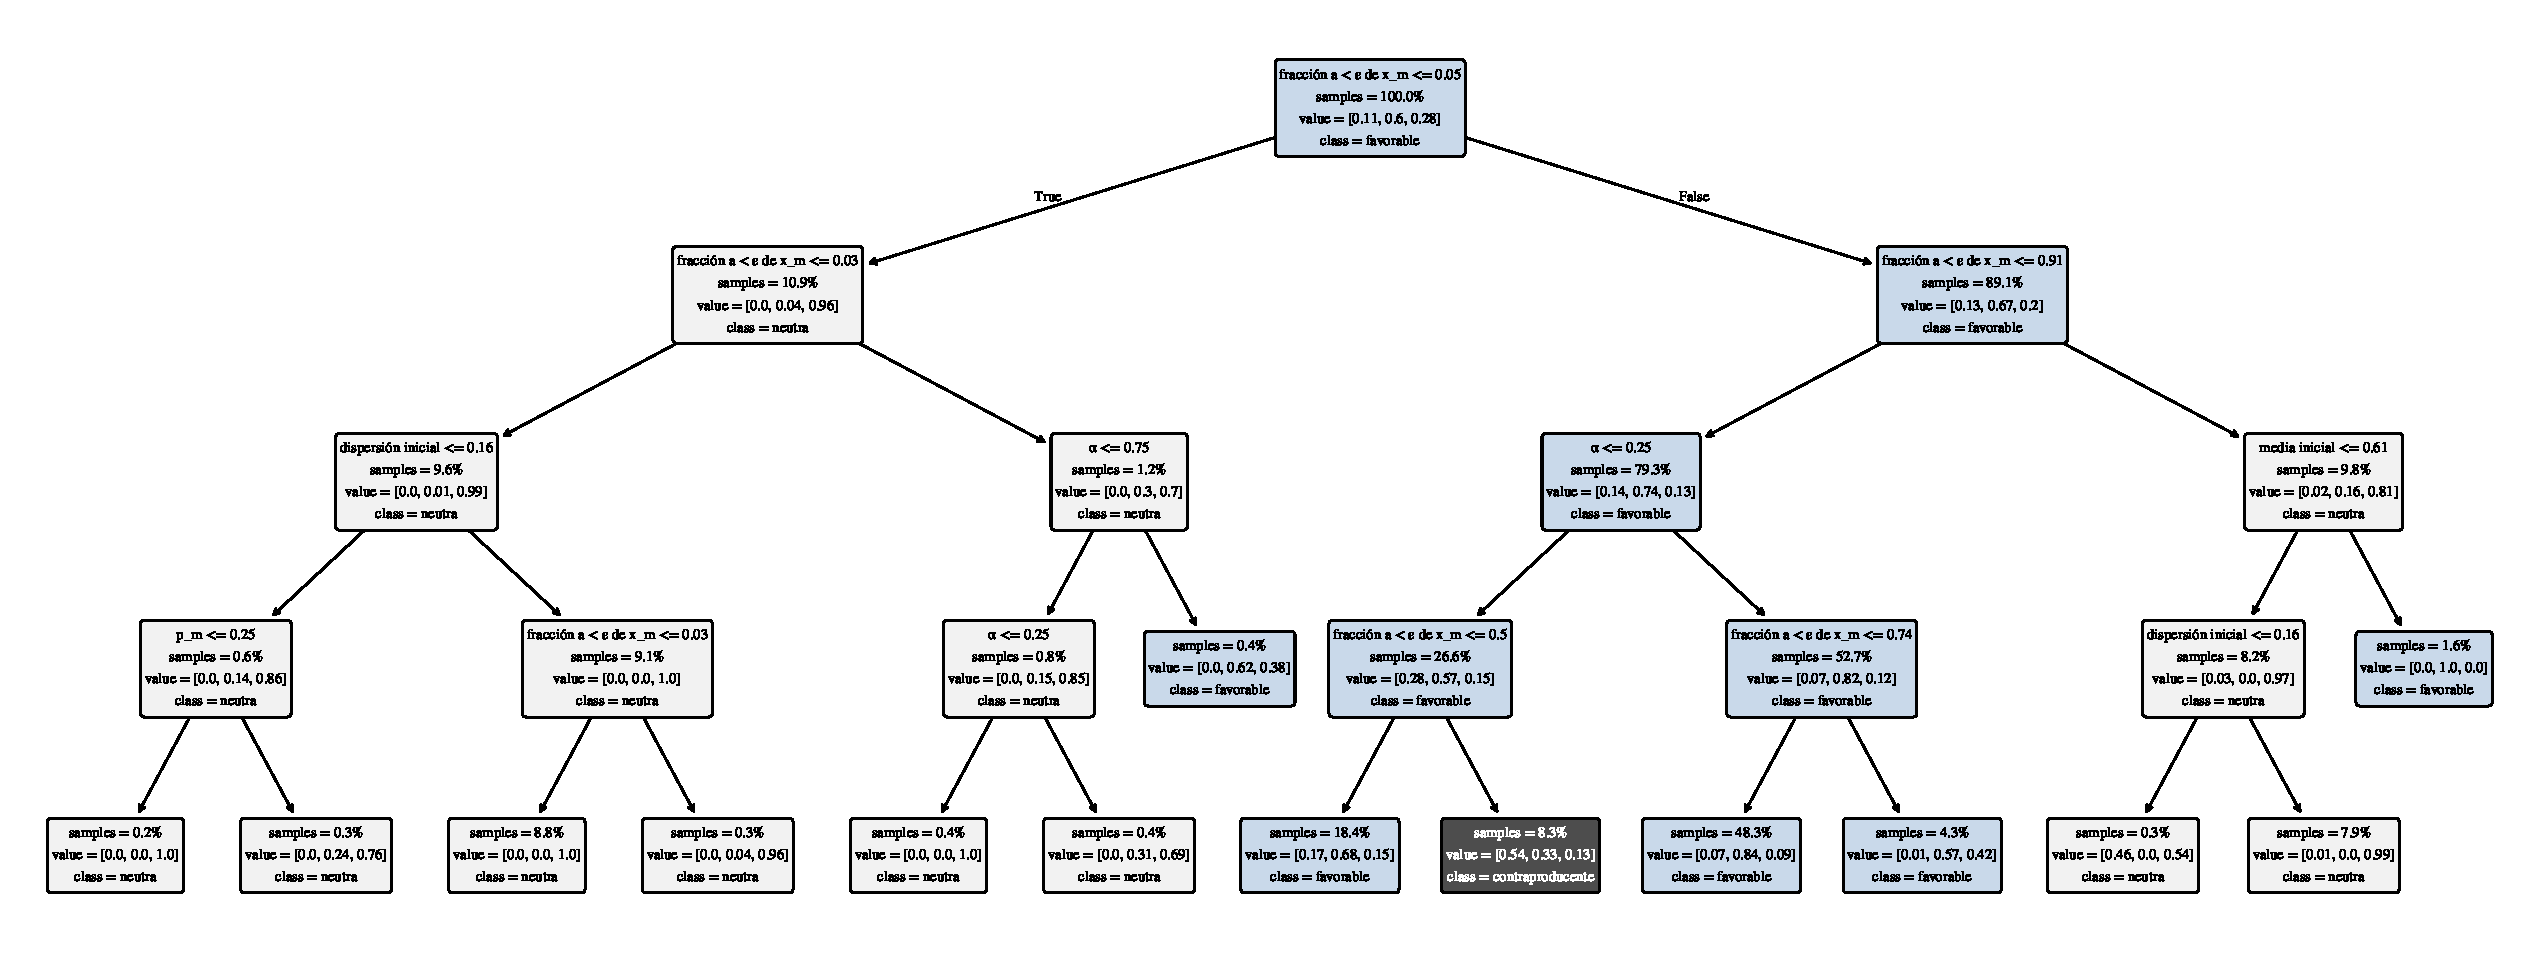
\includegraphics[width=\textwidth]{arbol_decision}
	\caption{Árbol de decisión con máximo 4 preguntas. Cada caja dice la pregunta, qué fracción de las
	corridas llega ahí, la proporción de cada etiqueta (contraproducente, favorable, neutra) y la etiqueta
	que asigna. Si la respuesta es sí (\emph{True}) se va a la izquierda. ``Fracción a $<\epsilon$ de
	$x_m$'' es la fracción de personas que al inicio ya está dentro del alcance de la campaña.}
	\label{fig:arbol}
\end{figure}

\begin{thebibliography}{9}
\setlength{\itemsep}{3pt}
\bibitem{Pansanella2023}
V. Pansanella, A. Sîrbu, J. Kertesz and G. Rossetti, \emph{Mass media impact on opinion evolution in biased digital environments: a bounded confidence model}, Scientific Reports \textbf{13} (2023) 14600.
\end{thebibliography}

\end{document}
